% This template has been tested with LLNCS DOCUMENT CLASS -- version 2.20 (10-Mar-2018)

% !TeX spellcheck = en-US
% !TeX encoding = utf8
% !TeX program = pdflatex
% !TeX TXS-program:compile = txs:///pdflatex/[--shell-escape]
% !BIB program = bibtex
% -*- coding:utf-8 mod:LaTeX -*-

% German documents: pass ngerman as class option
% \documentclass[ngerman,runningheads,a4paper]{llncs}[2018/03/10]
% English documents: pass english as class option
\documentclass[ngerman,runningheads,a4paper]{llncs}[2018/03/10]

\usepackage{improved-lncs}
\usepackage{subcaption}

\newcommand{\iu}{{i\mkern1mu}}

\makeatletter
\newcommand*\bigcdot{\mathpalette\bigcdot@{.5}}
\newcommand*\bigcdot@[2]{\mathbin{\vcenter{\hbox{\scalebox{#2}{$\m@th#1\bullet$}}}}}
\makeatother

\begin{document}

\title{Subsurface scattering: Kombination von Theorie und Implementierungstechniken am Beispiel des realistischen Renderns von Haut}
%If Title is too long, use \titlerunning
\titlerunning{Realitische Echtzeitdarstellung von Haut}

%Single insitute
\author{Dennis Grabowski, B.Sc.}
%If there are too many authors, use \authorrunning
\authorrunning{D. Grabowski}

\institute{Hochschule Hannover, Ricklinger Stadtweg 120, 30459 Hannover, Germany\\
\email{dennis.grabowski@stud.hs-hannover.de}\\
\url{https://f4.hs-hannover.de/}}

\maketitle

\begin{abstract}

Unter dem typischen Phong-Modell ist es schwer, verschiedenste Materialien wie Marmor, Wachs, Blätter oder Haut realistisch dar\-zu\-stellen.
Zugrunde liegt, dass das Phong-Modell nur ein empirisches Model ist und keineswegs ein physikalisch exaktes Modell darstellt, wodurch verschiedenste physikalische Effekte schlichtweg nicht nachstellbar sind.
Diese Ausarbeitung wird ausleuchten, welche Schwierigkeiten sich dabei ergeben, Haut realistisch darzustellen und welche physikalischen Konzepte nötig sind, um diesen Realismus wiedergeben zu können.
Haut als Medium bietet sich besonders an, um an diese fortgeschrittenen Beleuchtungsmodelle heranzugehen, da jedem Leser ein realistisches Erscheinungsbild dieser bekannt ist.
Hierfür wird zunächst aufgezeigt, wie Licht mit Haut interagiert, um die physikalischen Grundlagen der sogenannten Volumenstreuung (engl. subsurface scattering) kennenzulernen.
Anschliessend werden bestehende Techniken angeschnitten, die dieses physikalische Phänomen auf verschiedenste Weisen implementieren.
Durchleuchtet wird die sogenannte \enquote{Texture-space Diffusion}, welche bereits für den Film \enquote{The Matrix} verwendet wurde und von NVIDIA's d'Eon und Luebke für ein Echtzeit-Rendering-System adaptiert wurde.
Diese Technik verwendet die bidirektionale Reflexionsverteilungsfunktion von Kelemen und Szirmay-Kalos, um eine realistische Oberflächenreflexion zu simulieren, sowie Diffusionsprofile und Translucent Shadow Maps, um die Auswirkungen des Subsurface Scattering auf dem Hautmaterial nachzuahmen.

\end{abstract}

\begin{keywords}
  Computergrafik, Physikalisch-basiertes Rendering, Bidirektionale Reflexionsverteilungsfunktions (BRDFs), Subsurface scattering (deutsch Unterirdische Streuung/Volumenstreuung), Diffusionsprofile, Translucent shadow maps
\end{keywords}

\section{Einleitung}
\label{sec:intro}

Mithilfe des typischen Blinn-Phong-Modells ist es schwer, Materialien wie Marmor, Wachs, Blätter oder Haut realistisch darzustellen. Das basiert auf dem Fakt, dass dies ein empirisches Modell ist, welches keineswegs versucht, in der Lage zu sein, alle physikalische Phänomene nachstellen zu können.
Um die zuvorgenannten Materialien realistisch darstellen zu können, sind komplexere, physikalisch-fundierte Konzepte wie beispielsweise das \enquote{Subsurface Scattering}, zu deutsch \enquote{Volumenstreuung}, erforderlich.
Dieses physikalische Phänomen beschreibt, wie Licht mit einem Objekt interagiert, nachdem es von diesem gebrochen, aber nicht reflektiert wird.

Das Ziel dieser Ausarbeitung ist es, das Prinzip der Volumenstreuung vorzustellen und dem Leser einen Überblick über mögliche Techniken zu verschaffen, um dieses Phänomen durch vorhandene Techniken der Computergrafik entweder physikalisch korrekt darzustellen oder zu approximieren.

Hierfür werden zunächst die physikalischen Grundlagen aufgefrischt, die nötig sind um die Volumenstreuung zu verstehen, und erklärt warum der Aufbau des Objekts einen Unterschied für die Streuung darstellen kann.
Damit diese Erklärung relativ simpel bleiben kann, konzentriert sich diese Ausarbeitung auf Objekte, deren Oberfläche aus dem Material \enquote{Haut} bestehen.
Haut eignet sich besonders in diesem Kontext, da jedem Leser eine realistische Repräsentation dieses Materials wohl vertraut ist. Ferner sind Menschen darauf evolutionstechnisch trainiert, die feinsten Nuancen und Details instinktiv zu erkennen.

Nach Bewältigung der physikalischen Grundlagen werden 4 der bekanntesten realistischsten Haut-Render-Techniken vorgestellt, wovon der Fokus dieser Ausarbeitung auf der sogenannten \enquote{Texture-Space Diffusion} liegt, die bereits zum Film \enquote{The Matrix} Einsatz gefunden hat, und von NVIDIA's \citet{efficient-human-skin-rendering} angepasst wurde, um in einem Echtzeit-Renderer verwendet werden zu können.

Diese Technik kombiniert die Anwendung der \enquote{bidirektionalen Reflexions\-verteilungs\-funktion} von Kelemen und Szirmay-Kalos mit der Anwendung von sogenannten \enquote{Diffusionsprofilen} und \enquote{Translucent Shadow Maps}, um die realistische Darstellung von Haut zu ermöglichen.

Nachfolgend werden Bilder verschiedenster Implementationen sowie aktuellere Ergebnisse von \enquote{Offline-Renderern} miteinander verglichen, um die Wirkung dieser Beleuchtungsmodelle besser einschätzen zu können.

\section{Physikalische Grundlagen der Volumenstreuung}

Um die Volumenstreuung vollständig verstehen zu können, bedarf es zunächst einer Auffrischung bezüglich der physikalischen Eigenschaften des Lichts und der generellen Lichtbrechung.

Licht ist eine Welle, die sich innerhalb eines Mediums (oder auch innerhalb eines Vakuums) geradlinig in eine Richtung fortbewegt.
In dieser Ausarbeitung bezeichnet Licht immer das für das menschliche Auge sichtbare Licht mit einer Wellenlänge von ungefähr 380 bis 800 nm. Andere elektromagnetische Strahlungen werden somit ignoriert.

Trifft eine Lichtwelle auf ein anderes Medium, so erfährt es den Effekt der \enquote{Streuung} - es teilt sich in verschiedene Richtungen auf. Dadurch ändert sich nicht die gesamte Intensität, jedoch teilt sich die Intensität auf mehrere Lichtstrahlen auf.
Dabei werden die Lichtstrahlen entweder von der Oberfläche reflektiert, von der Oberfläche gebrochen oder absorbiert.
Die genauen Effekte des Eintreffens auf die Oberfläche eines neuen Mediums hängen von mehreren Faktoren ab: dem Einfallswinkel des Lichts auf die Oberfläche des Objekts, der Beschaffenheit der Oberfläche und dem sogenannten \enquote{Brechungsindex}.

Da diese Ausarbeitung darauf abzielt, die Volumenstreuung zu erklären, wird von einer näheren Erklärung der Auswirkungen von Einfallswinkeln sowie Oberflächenbeschaffungen abgesehen, da diese sich eher auf eine Reflexion auswirken.

Der Brechungsindex beschreibt das Verhältnis der Wellenlänge des Lichts im Vakuum zur Wellenlänge im Material und somit auch das Verhältnis der Phasengeschwindigkeit des Lichts im Vakuum zu der in dem betrachteten Material.
Es ist somit eine optische Eigenschaft eines Materials.
Besonders interessant ist die mathematische Darstellung dieses Index als komplexe Zahl: $$ \underline{n} = n + \iu * K$$
Der reelle Teil $n$ der komplexen Zahl beschreibt hierbei den Einfluss des Materials auf die Phasengeschwindigkeit des Lichts, wie stark das Licht durch das Material bei der Brechung verlangsamt wird, während der imaginäre Teil $\iu * K$ den Massenschwächungskoeffizienten beschreibt, ergo wie stark die Intensität des Lichts beim Propagieren durch das Material gedämpft wird.
Zusätzlich lässt sich mithilfe des Snelliussches Brechungsgesetzes und des Brechungsindex der Ausfallswinkel des gebrochenen Lichtstrahls in Relation zu dem Einfallswinkel des einfallenden Lichtstrahls berechnen.
Dadurch kann vorhergesagt werden, welchen Weg ein gebrochener Lichtstrahl innerhalb eines neuen Mediums nehmen wird - was eine hilfreiche Eigenschaft für das Rendern solcher gebrochenen Lichtstrahlen ist.

Was genau jedoch einem gebrochenen Lichtstrahl widerfährt, hängt von der Art des ihn brechenden Mediums ab.
Metalle absorbieren die gebrochenen Lichtstrahlen vollständig und wandeln diese in Hitze um.
Nicht-Metalle, sogenannte Dielektrika, wiederum verhalten sich wie reguläre Medien - innerhalb dieser interagieren gebrochene Lichtstrahlen mit den Partikeln des Materials wie Lichtstrahlen, die auf die Oberfläche eines Mediums treffen - auch diese können absorbiert, wieder reflektiert, schlichtweg aus dem Objekt wieder emittiert werden oder sogar streuen.
Hierbei können die Dielektrika-Medien nach der Menge an unterschiedlichen Brechungsindexen gruppiert werden, wodurch sich die Auswirkungen eines gebrochenen Lichtstrahls für eine Vielzahl von Materialien zusammenfassen lassen.
Transparente Medien, beispielsweise Glas oder Wasser, haben nur einen gleichbleibenden Brechungsindex, erlauben keine nennenswerte Absorption und lassen das Licht ohne Brechung durch sie passieren.
Homogene Medien, beispielsweise Bier, Kaffee, Wein oder Milch, haben zwar auch nur einen gleichbleibenden Brechungsindex, jedoch absorbieren sie eine signifikante Menge des Lichts. Dadurch ändert sich nicht die Richtung, allerdings die Intensität des Lichts, wodurch sich der Farbunterschied dieser Medien erklären lässt.
Heterogene Medien, beispielsweise Holz, Stein, Plastik, wiederum haben basierend auf strukturellen Änderungen mehrere unterschiedliche Brechungsindexe. Diese strukturellen Änderungen basieren entweder auf der Unreinheit eines Materials - Luftblasen, mikroskopisch, kleine Fremdpartikel oder ähnliches - oder basieren auf der Unterteilung in verschiedene Schichten, die wiederum alle aus verschiedenen Materialen bestehen.
Ändern sich die Brechungsindexe eines heterogenen Mediums stetig, so wird das Licht gebogen.
Ändern sich diese jedoch abrupt, so streuen die Lichtstrahlen an jedem neuen Brechungsindex.
Hierbei ändert sich die Richtung sowie die Intensität der Lichtstrahlen, jedoch kann es auch zu einer Absorption der Lichtstrahlen kommen. \cite{hoffman2013background}

Problematisch wird jedoch die Betrachtung von gebrochenen Lichtstrahlen im Falle einer komplexeren Materialbeschaffenheit eines Objekts, beispielsweise Haut - dem Fokus dieser Ausarbeitung.
Verschiedene Hautschichten bestehen aus verschiedenen Materialien, wodurch sich verschiedene, abrupt-wechselnde Unterschiede in den Brechungsindexen ergeben.
Jede neue Hautschicht absorbiert, reflektiert, bricht und streut das Licht also auf ihre eigene Art und Weise.

Diese Streuung unterhalb der Oberfläche eines Objekts nennt sich \enquote{Subsurface scattering} oder zu deutsch \enquote{Volumenstreuung}.

\section{Subsurface scattering}
\label{sec:subsurface}

\begin{figure}
  \centering
  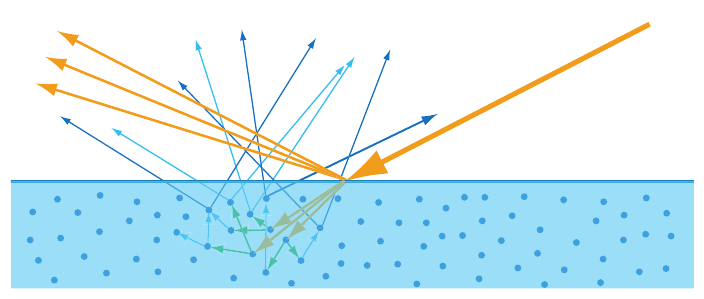
\includegraphics[scale=0.4,keepaspectratio]{./images/subsurface-scattering-illustration.jpg}
  \caption{Darstellung der Volumenstreuung in dielektrischen Materialien. Quelle: \cite{real-time-rendering}}
  \label{fig:subsurface-scattering}
\end{figure}

Die Volumenstreuung ist ein physikalisches Phänomen, welches beschreibt, was mit gebrochenen Lichtstrahlen innerhalb eines Objekts passiert.
Hierbei treffen an der Oberfläche des Objekts gebrochene Lichtstrahlen innerhalb des Objekts auf weitere, abrupte Änderungen, wodurch die gebrochenen Lichtstrahlen ferner in eine Vielzahl von Lichtstrahlen mit potentiell unterschiedlichen Intensitäten und potentiell allen möglichen Richtungen aufgeteilt werden.
Die Verteilung dieser Streuung hängt von dem Typen des Materials ab und ist häufig nicht uniform.

In Grafik \ref{fig:subsurface-scattering} wird dieser Effekt nochmal verdeutlicht. Der orangene Pfeil, der von oben rechts auf das neue Medium fällt, ist ein einzelner Lichtstrahl, der bei der Interaktion an der Oberfläche des Mediums streut. Ein Teil, erkenntlich durch die drei kleineren, orangenen Pfeile, die sich von dem Medium wieder entfernen, wird direkt von der Oberfläche reflektiert.
Die restlichen Lichtstrahlen werden mit der verbleibenden Intensität in verschiedenste Richtungen innerhalb des Mediums gebrochen und interagieren hierbei mit einzelnen Partikeln, die einen anderen Brechungsindex haben, als das Medium, in welchem sie sich befinden.
Verfolgt man die grünen Pfeile, so fällt auf, dass einige Lichtstrahlen vollständig von dem Medium absorbiert werden, wobei andere wieder von dem Objekt emittiert werden.
Hierbei müssen die wieder emittierten Lichtstrahlen nicht aus dem selben Punkt austreten, aus welchem sie ins Medium getreten sind. In der Grafik \ref{fig:subsurface-scattering-different-exit-point} wird nochmal verdeutlicht, wie stark der Austrittspunkt mancher der dargestellten Lichtstrahlen von dem Eintrittspunkt des ersten, einfallenden Lichtstrahls abweichen.

\begin{figure}
  \centering
  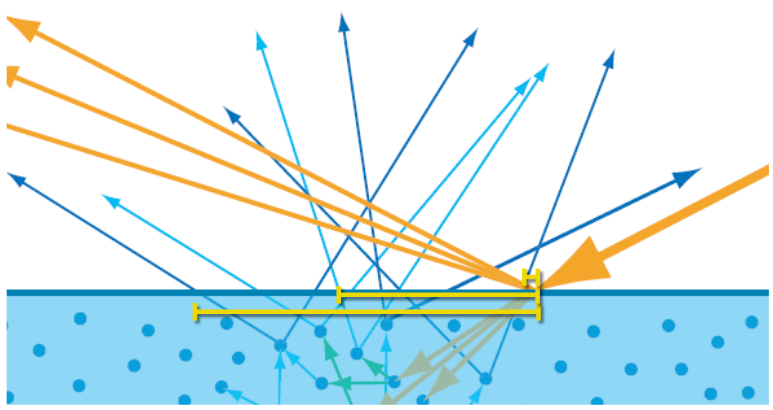
\includegraphics[scale=0.3,keepaspectratio]{./images/subsurface-scattering-distance-difference.jpg}
  \caption{Distanzunterschiede sind zwischen den Austrittspunkten und dem Eintrittspunkt zu erkennen. Quelle: \cite{real-time-rendering}}
  \label{fig:subsurface-scattering-different-exit-point}
\end{figure}

Aus den Grafiken \ref{fig:subsurface-scattering} und \ref{fig:subsurface-scattering-different-exit-point} ist ebenfalls erkenntlich, dass Lichtstrahlen unterschiedlich oft innerhalb eines Mediums streuen, bevor sie wieder von diesem Medium emittiert werden.
Man unterscheidet hierbei zwischen dem \enquote{Single-bounce scattering} und dem \enquote{Multiple-bounce scattering}; frei übersetzt der einfachen Streuung und der mehrfachen Streuung.

\subsection{Konzeptionelle Adaptation der Volumenstreuung in der Computergrafik}

Appliziert man die eben gewonnenen Erkenntnisse auf die Computergrafik, so kann man die Distanzunterschiede der neu-emittierten Lichtstrahlen in Abhängigkeit von Pixelgrössen darstellen, wie in Grafik \ref{fig:subsurface-scattering-pixel-considerations} dargestellt ist.

\begin{figure}
  \centering
  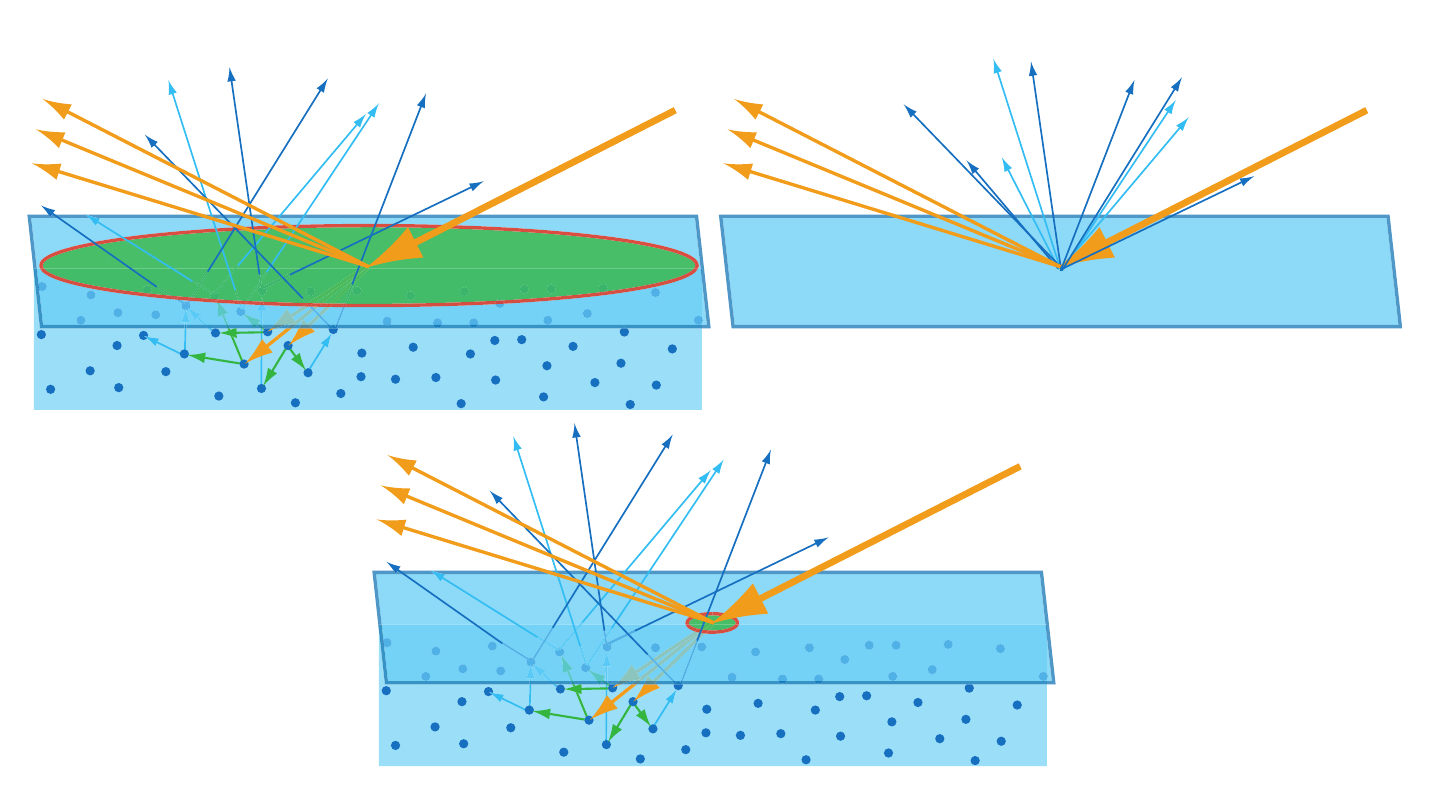
\includegraphics[scale=0.2,keepaspectratio]{./images/subsurface-scattering-pixel-considerations.jpg}
  \caption{Distanzunterschiede der neu-emittierten Lichtstrahlen in Abhängigkeit verschiedener Pixelgrössen. Quelle: \cite{real-time-rendering}}
  \label{fig:subsurface-scattering-pixel-considerations}
\end{figure}

Innerhalb dieser Grafik ist das bereits vorgestellte Beispiel zur Volumenstreuung um einen grünen Kreis erweitert worden, der die Grösse eines Pixels signalisieren soll.
Die linke Darstellung in der ersten Reihe zeigt somit ein Szenario, bei welchem die Distanz der Austrittspunkte der neu-emittierten Lichtstrahlen in Relation zu dem Eintrittspunkt des einfallenden Lichtstrahls kleiner ist als ein Pixel.
Dieses Szenario wird in der rechten Darstellung der ersten Reihe  vereinfacht dargestellt, in dem ein Renderer die Austrittspunkte in der Mitte des Pixels simuliert.
Die untere Abbildung zeigt den anderen Fall: Die Austrittspunkte sind ausserhalb des Pixels des einfallenden Lichtstrahls.

Diese Szenarien werden als lokale und globale Volumenstreuung kategorisiert.
Bei einer lokalen Volumenstreuung kann die Beleuchtung jedes Pixels individuell berechnet werden.
Dadurch ermöglichen sich beispielsweise Performancegewinne durch Parallelität oder den Wechsel zu dieser Methode beim Rendern von weit entfernten Charakteren.
Implementiert werden lokale Volumenstreuungen normalerweise durch eine \enquote{Lambert'sche  bidirektionale Reflektionsverteilungsfunktion}, die in der Lage ist, diffuse Reflektion mathematisch darzustellen. Die Lambert'sche BRDF hat normalerweise folgende mathematische Definition: $f_{Lambert}(l, v) = \rho_{ss} / pi$ \cite{real-time-rendering}
Hierbei beschreiben $l$ den Einheitsvektor des einfallenden Lichtstrahles, $v$ den ausgehenden Einheitsvektor der Blickrichtung und $\rho_{ss}$ die \enquote{Untergrundalbedo}.
Die Albedo eines Dielektrika ist definiert als das Verhältnis von der Radiosität, die von dem bestrahlten Objekt ausgeht, zu der Bestrahlungsstärke, die auf die Oberfläche einfällt.
Sie kann einen Wert zwischen 0 (jegliche Lichtstrahlen werden absorbiert) und 1 (keine Lichtstrahlen werden absorbiert) belegen, und hängt ferner von der Wellenlänge des jeweiligen Lichtstrahls ab, weshalb sie oftmals als RGB-Vektor modelliert wird.\cite{real-time-rendering}

Die eben vorgestellte mathematische Definition berücksichtigt allerdings nicht, dass die Lichtstrahlen, welche von der Oberfläche reflektiert werden, nicht für die Volumenstreuung nutzbar sind.
Eine typische Verbesserung wäre daher, den Fresnelschen Effekt zu beachten, welcher impliziert, dass bei einer Oberflächenreflexion sich die Menge an direkten Lichtstrahlen erhöhert und die Menge an diffusen Lichtstrahlen abnimmt, wenn zunehmend schrägere Einfallswinkel betrachtet werden.
Mathematisch lässt sich dies wie folgt ausdrücken:
$f_{diff}(l, v) = (1 - F(n, l)) * \rho_{ss} / pi$ \cite{real-time-rendering}
Hier beschreibt $n$ die typische Oberflächennormale.

Typischerweise ignorieren diese BRDFs die Einflüsse anderer Pixel, wodurch sie sich nicht bei einer Darstellung mit globalen Volumenstreuung eignen.
Bei einer globalen Volumenstreuung kann die Beleuchtung jedes Pixels potentiell die Beleuchtung jedes anderen Pixels des Bildes beeinflussen.
Diese Streuungen werden üblicherweise durch \enquote{globale Beleuchtungsmodelle} wie beispielsweise \enquote{Raytracern} dargestellt.
Auch einer der Vorreiter der realistischsten Haut-Render-Techniken, der BSSRDF von \citet{spectral-bssrdf-human-skin}, bedient sich dieser Methodik.
Für eine realistische Repräsentation ist ein Beleuchtungsmodell, welches globale Volumenstreuung berücksichtigt, unumgänglich.
Jedoch haben diese gewaltige Performanceimplikationen, wodurch Annäherungen oder ähnliche \enquote{Tricks} angewendet werden müssen.

\subsection{Struktur der Hautschichten}

Bevor die Vorstellung verschiedener Techniken zum realistischen Rendering des Materials Haut sinnvoll erscheint, sollte zunächst untersucht werden, wie die menschliche Haut strukturiert ist und welche physikalischen Eigenschaften sie besitzt.

\begin{figure}
  \centering
  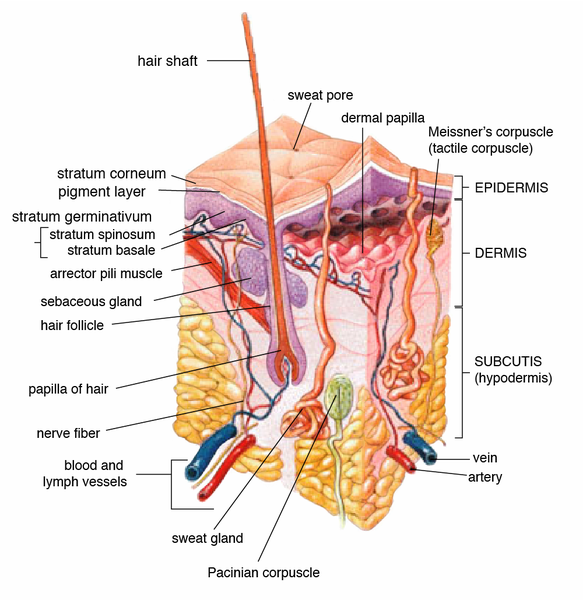
\includegraphics[scale=0.275,keepaspectratio]{./images/skin-layers-medical.png}
  \caption{Anatomisch korrekte Unterteilung der Haut in ihre Schichten. Quelle: \cite{anatomic-skin-model}}
  \label{fig:real-skin-layers}
\end{figure}

Die Grafik \ref{fig:real-skin-layers} zeigt eine medizinisch korrekte Darstellung der Zusammensetzung der unterschiedlichen Hautschichten. Die Haut ist somit ein heterogenes Medium.

Konzeptionell ist die Haut aufgeteilt in 3 Schichten: die Epidermis, die Dermis und die Hypodermis.
Direkt erkenntlich ist dass sich die unterschiedlichen Schichten, keineswegs das Volumen der Haut uniform aufteilen.
Die Hypodermis und die Dermis machen einen höheren Anteil der Haut aus, während die Epidermis hingegen die äusserste Schicht bildet, und somit als erstes mit einfallenden Lichtstrahlen interagiert.
In der Grafik leider nicht dargestellt ist das Sebum, eine ölige Substanz, die sich über Hautoberfläche zieht und für ihren Glanz sorgt.
Ferner bestehen alle Schichten aus unterschiedlichen Materialien und sind von unterschiedlichen \enquote{Fremdpartikeln} durchzogen.
Haare oder Schweisporen strecken sich von der Hypodermis bis hin zur Epidermis.
Feine Venen und Arterien ziehen sich durch alle Schichten, um die Blutgefässe der Haut mit ausreichend Blut versorgen zu können.
All diese Materialien verursachen, dass gebrochene Lichtstrahlen in die unterschiedlichsten Richtungen mit den unterschiedlichsten Intensitäten gestreuut werden.
Eine exakte Repräsentation dieses Modells erweist sich daher als unhandlich für das realistische Rendering der Haut.

Laut \citet{tuchin2015tissue} werden \textasciitilde{}6\% des einfallenden Lichts direkt an der Hautoberfläche dank des Sebums reflekiert, während die restlichen \textasciitilde{}94\% innerhalb der Haut der Volumenstreuung unterliegen.
Für die reflektierten Lichtstrahlen ist hauptsächlich das Sebum verantwortlich.
Die Stratum Corneum ist hingegen höchst streuend, wodurch viele, multiple Streuungen stattfinden.
Ferner haben alle Bestandteile unterhalb der Dermis keinen nennenswerten Effekt auf die fürs menschliche Auge wahrgenommene Erscheinung \cite{tuchin2015tissue}.

Erforderlich ist somit ein Beleuchtungsmodell, dass den geringen Anteil der direkt reflektierten Lichtstrahlen und deren richtige Verteilung korrekterweise wiedergeben kann, sowie in der Lage ist eine globale Volumenstreuung zu simulieren.
Simulieren bedeutet hier, dass nicht unbedingt eine wissenschaftlich umfassende Präsentation erforderlich ist.
Möglich ist auch eine Approximation.

\section{Texture-Space Diffusion}
\label{sec:texture-space}

Die sogenannte \enquote{Texture-Space Diffusion} ist eine von NVIDIA's \citet{efficient-human-skin-rendering} fortgeführte Methodik, die sich auf den Ergebnissen von \citet{realistic-human-face-rendering-matrix} stützt.
Diese versuchten für die Trilogie \enquote{The Matrix} eine Rendertechnik zu finden, mithilfe welcher sie in der Lage sind, Haut auch realistisch im Falle des \enquote{Morphing} des \enquote{Agent Smith} darstellen zu können.
Während ihrer Forschung fiel ihnen aufgefallen, dass ein realistisches Ergebnis ohne Volumenstreuung nicht möglich ist.
Die bis dato veröffentlichten Techniken waren jedoch entweder rechnerisch zu kostspielig oder lieferten eher enttäuschende Ergebnisse.
Daher entwickelteten \citet{realistic-human-face-rendering-matrix} die Beleuchtungstechnik, \enquote{Texture-Space Diffusion}, die die Effekte der Volumenstreuung in Falle der menschlichen Haut approximiert.

Diese Approximation basiert auf Forschungsergebnissen von \citet{stam1995multiple} und \citet{spectral-bssrdf-human-skin}, die später von \citet{ma2007rapid} erweitert wurde.
\citeauthor{stam1995multiple}'s Forschung ergab, dass multiple Volumenstreuungen als Zerstreuungen modelliert werden können.
Das Beleuchtungsmodell, das aus der Forschung von \citeauthor{spectral-bssrdf-human-skin} entstand, griff diese Idee auf, um eine analytische BSSRDF speziell für das Rendern von Haut abzuleiten; eine BRDF für den Fall einer globalen Volumenstreuung generalisiert.

Im Rahmen des vorgestellten wissenschaftlichen Artikels \enquote{Efficient Rendering of Human Skin} von \citet{advanced-realtime-skin-rendering} wird diese Technik innerhalb eines vollständiges Beleuchtungsmodelles verwendet, welches speziell zum Echtzeit-Rendern realistischer, menschlicher Haut erstellt wurde.

Dieses Beleuchtungsmodell, welches folgend detallierter erklärt wird, besteht aus:

\begin{itemize}
  \item Der BRDF von Kelemen und Szirmay-Kalos, um Lichtstrahlen zu modellieren, die direkt von der Hautoberfläche reflektiert werden,
  \item Diffusionsprofilen, die innerhalb der Texture-Space-Diffusion verwendet werden,
  \item und modifizierte \enquote{Translucent Shadow Maps} \citep{translucent-shadow-maps}, durch welche die korrekte Durch-/Beleuchtung dünnerer Hautpartien ermöglicht wird
\end{itemize}

Die vorgestellte Technik bezieht ihren Namen aus dem Fakt, dass die gesamte Simulation der Volumenstreuung in einer 2D-Texture des Objektmeshes unter Verwendung der UV-Parametrisierung erfolgt.

Im Folgenden wird davon abgesehen, alle Informationen des Papers \cite{efficient-human-skin-rendering} und des daraus entstandenen Artikels in der \enquote{GPU Gems 3} \cite{advanced-realtime-skin-rendering} jedesmal mit ihrer Quellenangabe zu versehen.

\subsection{Von der Hautoberfläche reflektierte Lichtstrahlen}
\label{sub:skin-surface-reflect}

Die Autoren \citeauthor{efficient-human-skin-rendering} verwenden für Lichtstrahlen, die direkt von der Hautoberfläche reflektiert werden, die BRDF von Kelemen und Szirmay-Kalos \cite{kelemen2001microfacet}.
Sie weichen von der Wahl der \enquote{Cook-Torrance}-BRDF, die in \citet{spectral-bssrdf-human-skin} verwendet wurde, ab und begründen diese alternative BRDF damit, dass die \enquote{Kelemen und Szirmay-Kalos}-BRDF signifikant weniger rechenintensiv sei, während sie ein ähnliches, visuelles Ergebnis liefert (Begründung ebenfalls in \cite{hoffman2013background} zu finden).
Diese BRDF ist allgemein mathematisch wie folgt definiert\footnote{Formel entnommen von \cite[p.~352]{real-time-rendering}, die ihrerseits \cite{kelemen2001microfacet} als Quelle angibt}: $$f_{diff}(l, v) = \rho_{ss} * \frac{(1 - R_{spec}(l))* (1 - R_{spec}(v))}{\pi * (1 - \overline{R_{spec}})}$$

Hier beschreibt $R_{spec}$ die direkt von der Oberfläche reflektierten Lichtstrahlen der BDRF (in der Literatur auch manchmal aus \enquote{direktionale Albedo} bezeichnet) und $\overline{R_{spec}}$ das Kosinus-gewichtete Integral der direktionalen Albedo über die Einheitshemisphäre, die sich mithilfe des Normalenvektors auf der Oberfläche bilden lässt.
Dies lässt sich dadurch erklären, dass potentiell jeder mögliche Einfallswinkel etwas Strahlungsstärke mit sich trägt.

Ferner wird innerhalb des Verfahrens die BRDF durch folgende Anpassungen berechnungseffizienter gestaltet.
$rho_{ss}$ (sowie $m$) nehmen vorbestimmte Werte, die einer Studie von \citet{weyrich2006analysis} entnommen werden können, an, um Berechnungsaufwand zu sparen.
Die Autoren geben darüber hinaus an, dass sie $\rho_{dt}$, eine \enquote{diffuse transmission function} vorberechnen, indem für verschiedene \enquote{Roughness}-Werte $m$ eine vorberechnete Beckmann-Verteilungs-Funktion angewandt wird und die Ergebnisse innerhalb einer 2D-Texture gespeichert werden.
Leider spezifizieren die Autoren nicht, wofür diese Funktion genau verwendet wird, ebenso konnten keine Informationen zu dieser \enquote{diffuse transmission function} und ihren Einsatz gefunden werden.
\\
\\
In Grafik \ref{fig:outlook-final-result-no-sss} (a) kann die gerenderte Haut betrachtet werden, wenn nur die BRDF von Kelemen und Szirmay-Kalos appliziert wird.

\subsection{Unter der Hautoberfläche streuende Lichtstrahlen}
\label{sub:skin-subsurface-reflect}

\subsubsection{Diffusionsprofile}
\label{sub:diffusion-profiles}

\begin{figure}
  \centering
  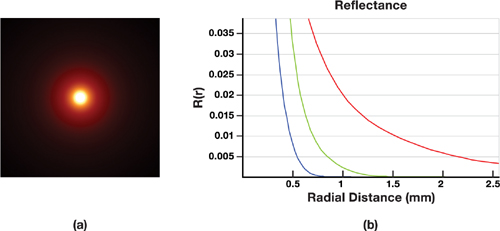
\includegraphics[scale=0.7,keepaspectratio]{./images/diffusion-profile-visualization}
  \caption{Visualisierung eines Diffusionprofiles durch die Durchführung des genannten physikalischen Experiments. Quelle: \cite{advanced-realtime-skin-rendering}}
  \label{fig:diffusion-profile-experiment}
\end{figure}

Um die Texture-Space Diffusion vollständig verstehen zu können, müssen wir zunächst das Konzept der \enquote{Diffusionsprofile} einführen.

Die Verteilung der gestreuten Lichtstrahlen tendiert in einem hochstreuendem Medium dazu isotrop zu sein.
Das bedeutet: Sobald Lichtstrahlen in ein Medium hinein gebrochen werden, ist es wahrscheinlich, dass diese an einer zufälligen Stelle wieder auszutreten, anstatt von einem weiteren Faktor, wie beispielsweise dem Einfallswinkel des originalen, einfallenden Lichtstrahls abhängig zu sein. \cite{hoffman2013background}
Diese Erkenntnis kommt von den Forschungsergebnissen von \citet{stam1995multiple}.
Ferner zeigten \citet{ma2007rapid}, dass die Lichtstrahlen, die durch die Volumenstreuung erzeugt werden und aus dem Objekt wieder emittieren, sich verhalten als würde man verwischte Oberflächennormalen nutzen.

Basierend auf diesen Erkenntnissen können Diffusionprofile genutzt werden, um die Volumenstreuung innerhalb eines Mediums zu messen.
Stellt man sich folgendes Experiment vor, wird solch ein Diffusionprofil eventuell greifbarer.
Grafik \ref{fig:diffusion-profile-experiment} (a) zeigt, wie eine Lichtquelle auf die Mitte einer Fläche in einem dunklen Raum strahlt.
Hierbei ist zu erkennen, dass sich um den weißen Punkt in der Mitte ein roter Schein gebildet hat.
Dieser Schein stellt die Lichtstrahlenstreuung innerhalb des Objekts dar, wobei einige in das Objekt gebrochene Lichtstrahlen, von dem Objekt an einer anderen Position als den einfallenden Lichtstrahl wieder austreten.
Ein Diffusionprofil kann daher als eine Art Funktion betrachtet werden, die die Lichtstreuungsverteilung beschreibt; sprich, wie viele Lichtstrahlen abhängig von dem Winkel und der Distanz des einfallenden Lichtstrahls an anderen Stellen austritt.
Hierbei besitzt jede Wellenlänge ihr eigenes Diffusionprofil, wie in \ref{fig:diffusion-profile-experiment} (b) erkenntlich wird.
Donner und Jenson \cite{spectral-bssrdf-human-skin} verwenden beispielsweise bis zu 150 verschiedene Diffusionprofil für ihre BSSRDF.

\subsubsection{Verwendetes Hautschichtenmodell}
\label{sub:skin-model}

\begin{figure}
  \centering
  \begin{subfigure}{.5\textwidth}
    \centering
    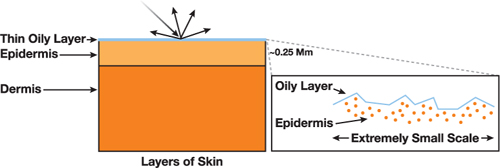
\includegraphics[scale=0.5,keepaspectratio]{./images/multilayer-skin-specular-reflection.jpg}
    \label{fig:multilayer-specular}
  \end{subfigure}%
  \begin{subfigure}{.5\textwidth}
    \centering
    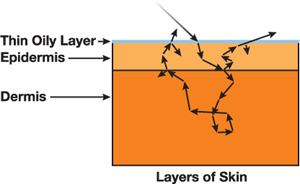
\includegraphics[scale=0.5,keepaspectratio]{./images/multilayer-skin-subsurface.jpg}
    \label{fig:multilayer-subsurface}
  \end{subfigure}
  \caption{Links: Oberflächenreflexion im 3-Schicht-Hautmodell, Rechts: Volumenstreuung im 3-Schicht-Hautmodell.\\\hspace{\textwidth}Quelle: \cite{advanced-realtime-skin-rendering}}
\end{figure}

In der Forschungsarbeit von Donner und Jensen \cite{spectral-bssrdf-human-skin} wurde ein Drei-Schichtenmodell für die Haut eingeführt, auf welchen die berechneten Diffusionprofile basieren.
Die Autoren \citeauthor{efficient-human-skin-rendering} stützen sich innerhalb dieser Ausarbeitung auf diese und berechnen für diese eine Approximation durch Summen mehrerer Gaußscher Verteilungsfunktionen.

\subsubsection{Approximation der Diffusionsprofile durch Gaußsche Summen}

Die dargestellten Kurven in Grafik \ref{fig:diffusion-profile-experiment} (b), ähneln der bekannten Gaußschen Verteilungsfunktion $e^{-r^{2}}$.
Die Autoren \cite{efficient-human-skin-rendering} machen sich diesen Fakt zur Nutze, um die Diffusionprofile, die Donner und Jensen \cite{spectral-bssrdf-human-skin} zu ihrem Drei-Schichtemodell berechnet haben, annäherungsweise zu bestimmen.
Dies erreichen sie mit einer Summe mehrerer Gaußschen Verteilungsfunktionen.
Das hat den Vorteil, dass Gaußsche Verteilungsfunktionen gleichzeitig zerteilbar sind, aber auch kreissymmetrisch sind.
Darüber hinaus gehen aus einer (mathematischen) Faltung wieder eine Gaußsche Verteilungsfunktionen hervor.

Diese werden danach summiert, um daraus die approximierten Diffusionprofile $R(r)$ zu erhalten: $R(r) = \sum\nolimits_{i=1}^k w_i * G(v_i, r)$.
Hierbei entschieden sich die Autoren, die Varianz der Gaußschichen Verteilungsfunktion $v$ wie folgt zu definieren:
$G(v, r) = \frac{1}{2 * \pi * v} * e^{\frac{-r^{2}}{2*v}}$
Der konstanter Faktor in der Gaußschen Varianz $\frac{1}{2 * \pi * v}$ wurde so gewählt, dass die applizierten Gaußschen Filter das Eingangsbild weder verdunkeln oder noch aufhellen.

Wie in Grafik \ref{fig:approximation} erkenntlich wird, nähern sich vier ($k$) summierte Gaußschen Verteilungsfunktionen erstaunlich gut an das Dipol-Diffusionprofil, welches Donner und Jensen \cite{spectral-bssrdf-human-skin} haben.

\begin{figure}
  \centering
  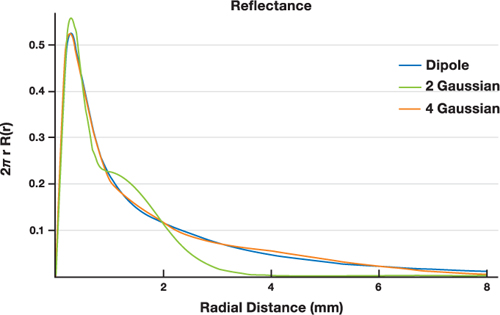
\includegraphics[scale=0.7,keepaspectratio]{./images/approximation-gaussians}
  \caption{Approximation der Dipol-Diffusionprofil von Donner und Jensen \cite{spectral-bssrdf-human-skin} durch Gaußsche Summen. Quelle: \cite{advanced-realtime-skin-rendering}}
  \label{fig:approximation}
\end{figure}

Aus der Zerteilbarkeit und der kreisförmigen Symmetrie entstehen ausserdem Performancegewinne; so lassen sich beispielsweise zwei eindimensionale Unschärfefilter über die x- und y-Koordinate berechnen, welche wiederum durch die Faltungseigenschaft danach simpel kombiniert werden können.

\subsubsection{Anwendung der Diffusionsprofil zur Simulation der Volumenstreuung}

\begin{figure}
  \centering
  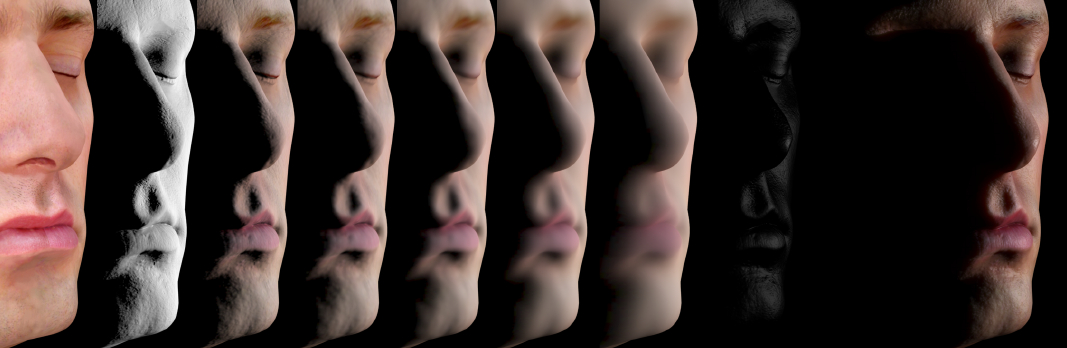
\includegraphics[scale=0.3,keepaspectratio]{./images/human-skin-final-rendering.jpg}
  \caption{Getrennte Darstellung der verschiedenen Renderschritte. Von links: Die Albedo, die zusammen mit der Bestrahlungsstärke kombiniert, die Bestrahlungsstärke der Volumenstreuung (dritter Schritt) ergibt. Diese wird durch die einzelnen Gaußschischen Diffusionprofile (Bild drei bis sieben) gefaltet, und produziert zusammen mit den reflektierten Lichtstrahlen das vollständige Ergebnis.\\\hspace{\textwidth}Quelle: \cite{efficient-human-skin-rendering}}
  \label{fig:whole-algorithm-rendered}
\end{figure}

Nun werden die Diffusionprofil innerhalb der \enquote{Texture-Space Diffusion} appliziert.
Ein überblick über den kompletten Algorithmus kann sich in Grafik \ref{fig:algorithm} verschafft werden.

\begin{figure}
  \centering
  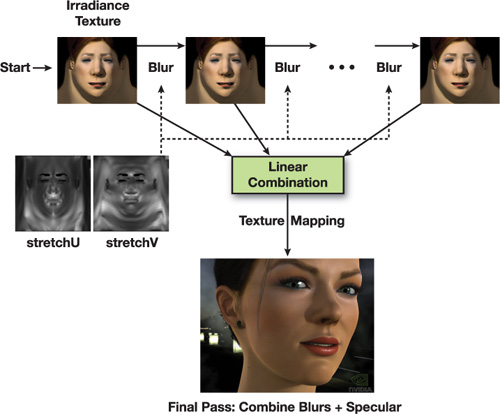
\includegraphics[scale=0.8,keepaspectratio]{./images/texture-space-algorithm.jpg}
  \caption{Ablauf des verbesserten \enquote{Texture-Space Diffusion}-Algorithmus. Quelle: \cite{advanced-realtime-skin-rendering}}
  \label{fig:algorithm}
\end{figure}

Hierfür wird zunächst das dreidimensionale Objektmesh durch das \enquote{UV unwrapping} in einem Vertexshader auf eine zweidimensionale Textur ausgeklappt.
Daraufhin wird die Bestrahlungsstärke (gesamte eingehende Lichtenergie) auf dieser Textur dargestellt.
Diese wird durch einen Fragmentshader berechnet, der das einfallende Licht aller Lichtquellen minus deren direkter Reflexion berechnet.
Nun wird jeder Gaußsche Unschärfefilter, der sich aus dem berechneten Diffusionprofil ergibt, separiert und in U- und sowie V-Koordinate des Texturraumes auf die Textur angewendet, die die Bestrahlungsstärke beinhaltet.
Daraufhin werden alle Gaußschen Filter linear miteinander kombiniert, und die reflektierten Lichtstrahlen aller Lichtquellen hinzugefügt, um das finale Bild zu erhalten. \\
Eine visuelle Darstellung mit den Ergebnissen jedes einzelnen Schritts kann auch in Grafik \ref{fig:whole-algorithm-rendered} betrachtet werden.

\begin{figure}
  \centering
  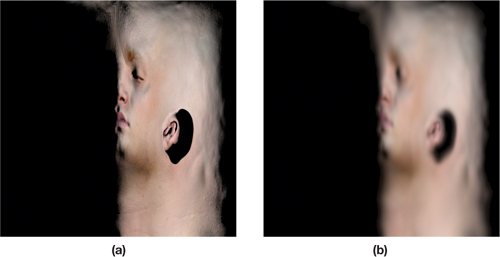
\includegraphics[scale=0.8,keepaspectratio]{./images/irradiance-texture-adrian.jpg}
  \caption{Auszug der Texturen, die die Bestrahlungsstärke darstellen. Links: initiale, bisher noch nicht verschwommene Textur, rechts: Ergebnis nach Applikation aller Gaußschen Unschärfefilter. Quelle: \cite{advanced-realtime-skin-rendering}}
\end{figure}

\begin{figure}
  \centering
  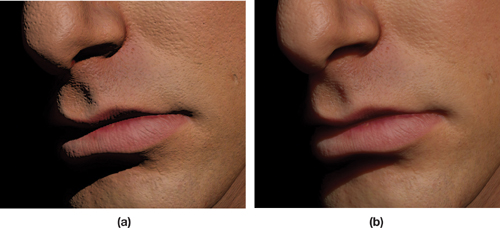
\includegraphics[scale=0.8,keepaspectratio]{./images/skin-rendering-with-without-sss.jpg}
  \caption{Ergebnis der \enquote{Texture-Space-Diffusion}-Technik, links ohne Volumenstreuung, rechts mit. Quelle: \cite{efficient-human-skin-rendering}}
  \label{fig:outlook-final-result-no-sss}
\end{figure}

\subsubsection{Korrektur der entstehenden Verzerrung durch das UV-Mapping}

Oben genannte Technik funktioniert hervorragend, solang ausschliesslich flache Oberflächen verwendet werden.
Werden allerdings geschwungene Oberflächen genutzt, so kommt es zu einer Verzerrung des Objektmeshes bei dem UV-Mapping, da die Distanzen der einzelnen Positionen auf der Texture nicht mit denen auf dem Mesh übereinstimmen.
Dieses Phänomen wird in Grafik \ref{fig:stretching} visualisiert.

\begin{figure}
  \centering
  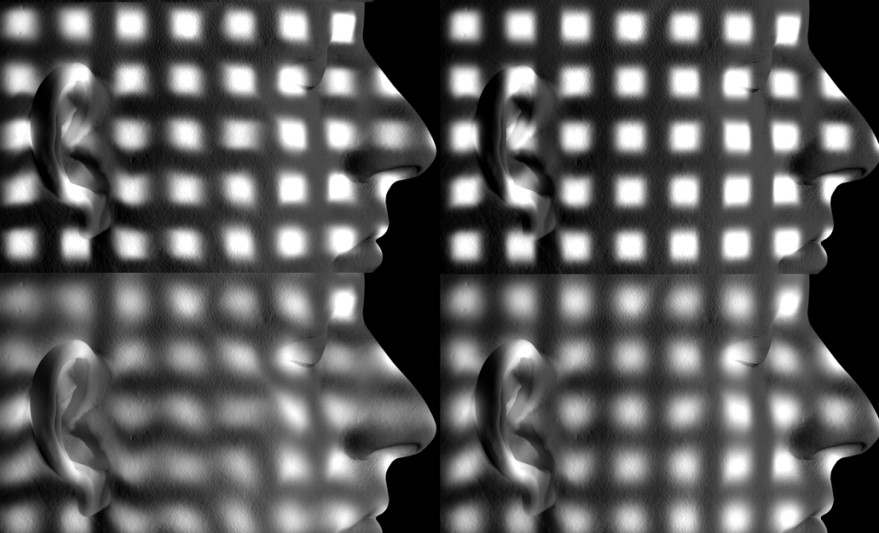
\includegraphics[scale=0.4,keepaspectratio]{./images/texture_space_stretch.jpg}
  \caption{Zur Verdeutlichung der entstehenden Verzerrung haben \citeauthor{efficient-human-skin-rendering} ein gleichmässiges Beleuchtungsmuster auf das Gesicht projeziert und danach den
  \enquote{Texture-Space Diffusion}-Algortihmus (untere Reihe) appliziert. Wie auf der linken Seite zu erkennen ist, entsteht eine Verzerrung dieses Musters. Bei Benutzung einer verzerrungskorrigierenden Texture (rechte Seite) wird Verzerrung deutlich korrigiert. Quelle: \cite{efficient-human-skin-rendering}}
  \label{fig:stretching}
\end{figure}

Diese Verzerrung umgehen \citet{efficient-human-skin-rendering} durch die Berechnung einer verzerrungkorrigierenden Textur.
Diese wird dynamisch für jedes einzelne Frame durch einen Fragmentshader erstellt, welcher auf dem zuvor via \enquote{UV unwrapping} entklappten Objektmesh aufbaut.
Hierfür werden die \enquote{World-Space} Koordinaten des Meshes innerhalb der Texturkoordinaten in zwei separate horizonale und vertikale \enquote{Verzerrungskorrekturtexturen} gespeichert.
Dieses Verfahren gibt eine effiziente Annäherung der auftreteten Verzerrung.

Wie in Grafik \ref{fig:algorithm} zu erkennen war, beeinflussen diese \enquote{Verzerrungskorrekturtexturen} die Gaußschen Unschärfefilter und werden bei jeder Anwendung der verschiedenen Filter mitverschwommen, um somit eine Korrektur der Verzerrung zu erreichen.

\subsection{Translucent Shadow Maps}
\label{sub:translucent-shadow-maps}

\begin{figure}
  \centering
  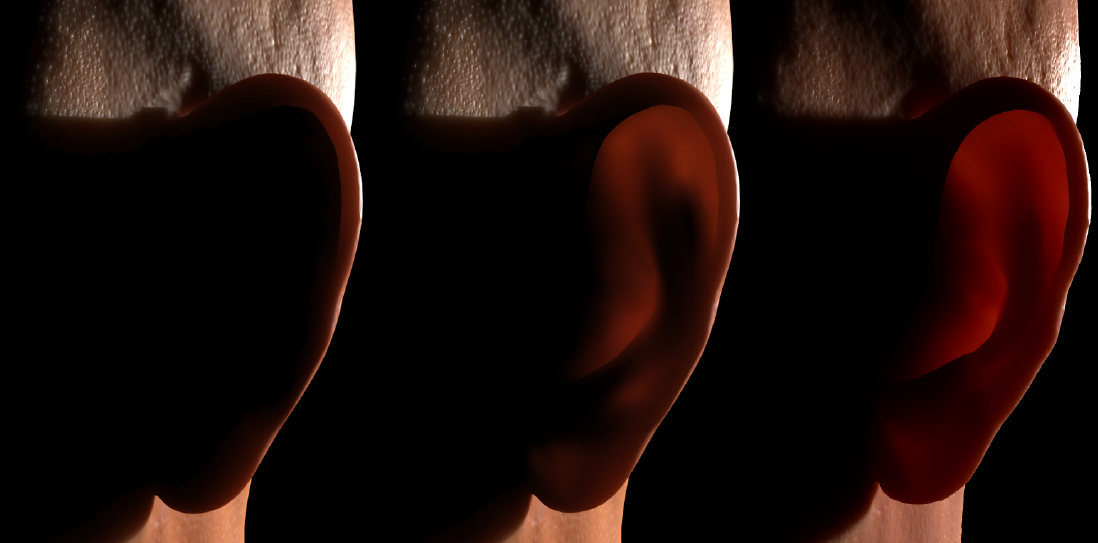
\includegraphics[scale=0.2,keepaspectratio]{./images/translucent-shadow-maps.jpg}
  \caption{
    Dünne Hautpartien gerendert durch verschiedene Techniken.\\\hspace{\textwidth}
    Links: Texture-Space Diffusion, Mitte: Rendering mit Translucent Shadow Maps, Rechts: spektrales BSSRDF-Modell von Jensen et al.\\\hspace{\textwidth}Quelle: \citet{efficient-human-skin-rendering}
  }
  \label{fig:tsm-result}
\end{figure}

Schwierig sind vor allem dünnere Hautpartien (beispielsweise Ohren, Nasenlöcher), durch welche (gebrochene, gestreute) Lichtstrahlen durchscheinen können.
Während \citet{realistic-human-face-rendering-matrix} hier für realistische Ergebnisse auf einen Raytracer zurückgreifen, hielten \citet{efficient-human-skin-rendering} diesen Ansatz für einen Echtzeitrenderer für zu rechenintensiv.
Um dennoch dünne Hautpartien realistisch darstellen zu können, verwenden \citeauthor{efficient-human-skin-rendering} sogenannte \enquote{Translucent Shadow Maps} von Dachsbacher und Stamminger \cite{translucent-shadow-maps}.

Problematisch ist, dass beim typischen \enquote{Texture-Space Diffusion}-Verfahren, globale Volumenstreuung übersehen werden können, wenn zwei Oberflächen des Objekts im dreidimensionalen Raum (Euclidean) zwar nahe beieinander liegen, aber sich weiter voneinander entfernt im zweidimensionalen Texturraum befinden.

D'Eon et al. modifizierten die Translucent Shadow Maps, um eine sehr effiziente Abschätzung der Volumenstreuung innerhalb dünner Hautregionen durch die Wiederverwendung von der berechneten, verschwommenen BeStrahlungsstärketexturen zu ermöglichen.
Typischerweise berechnen diese Translucent Shadow Maps die Tiefe, Bestrahlungsstärke sowie Oberflächennormale für jeden Pixel und speichern diese Werte an der Oberfläche, die sich am nähsten zur Lichtquelle befindet.
In der von \citeauthor{efficient-human-skin-rendering} modifizierten Variante hingegen, werden die U- und V-Koordinate sowie die Tiefe berechnet und gespeichert.
Dadurch ist möglich, für jede beschattete Oberfläche die Dicke des Objekts zu berechnen, und somit den Wert der Belichtungsstärke der gegenüberliegenden, zur Licht gewandten Oberfläche zu abzurufen.
In Grafik \ref{fig:tsm-darstellung} wird dieses Konzept nochmal visuell dargestellt.
Somit kann die Menge an Lichtstrahlen, die an dem beschatteten Punkt (in Grafik \ref{fig:tsm-darstellung} mit C betitelt), ermittelt werden.
Die genaue, korrekte Menge an austretenden Lichtstrahlen für den Punkt C zu berechnen, scheint allerdings schwieriger zu sein als eine Annäherung durch die Berechnung der austretenden Lichtstrahlen an Punkt B.
Hierfür entwickelteten \citeauthor{efficient-human-skin-rendering} eine Annäherung eines Diffusionprofils:
$$R(\sqrt{r^2 + d^2}) = \sum_{i=1}^{k} w_i * G(v_i, \sqrt{r^2 + d^2}) = \sum_{i=1}^{k} w_i * e^{\frac{-d^2}{v_i}} * G(v_i, \sqrt{r^2 + d^2}) $$

Diese Gaußsche Summe ermöglicht eine Transformation der Funktion von $\sqrt{r^2 + d^2}$ zu einer Funktion von $r$.
Dadurch kann die Menge an austretenden Lichtstrahlen an Punkt C annäherungsweise durch die austrentenden Lichtstrahlen an Punkt B berechnet, welcher für kleine Winkel, nahe genug an C ist.
Das Ergebnis dieses komplexen Verfahrens kann in Grafik \ref{fig:tsm-result} betrachtet werden.

\begin{figure}
  \centering
  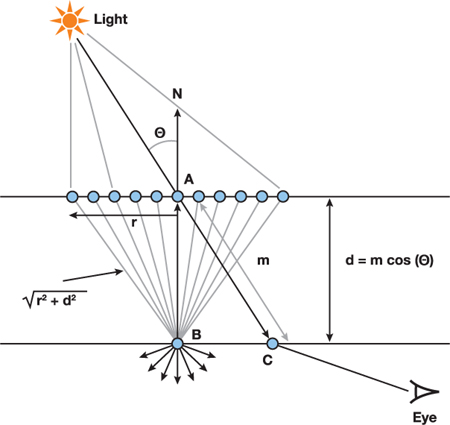
\includegraphics[scale=0.2,keepaspectratio]{./images/tsm-visualization.jpg}
  \caption{
    Darstellung der modifizierten Translucent Shadow Maps. Quelle: \citet{advanced-realtime-skin-rendering}
  }
  \label{fig:tsm-darstellung}
\end{figure}

\section{Konklusion und Ausblick}
\label{sec:outlook}

Das umfassende Ergebnis dieses Beleuchtungsmodells kann in Grafik \ref{fig:outlook-final-result} betrachtet werden.
In Grafik \ref{fig:outlook-final-result-no-sss} ist sichtbar, welchen Unterschied die simulierte Volumenstreuung im Kontext der verwendeten Technik macht.
Zweifelsohne lässt sich sagen, dass das Ergebnis sich sehen lässt.
Verglichen mit dem Ergebnis, dass sich durch die damalige \enquote{state-of-the-art} BSSRDF von Donner und Jensen \cite{spectral-bssrdf-human-skin}, rendern lässt, kann behauptet werden, dass sie ein sehr ähnliches Ergebnis erzielten.
\\

Jedoch ist die \enquote{Texture-Space-Diffusion} nicht ohne Limitationen oder Fehler.
Die Translucent Shadow Maps leiden laut \citet{efficient-human-skin-rendering} unter den Problematiken der regulären Shadow Maps; beispielsweise der Auswahl der angemessenen Auflösungen.
Darüber hinaus ist man zu der Benutzung einer kleinen Menge an vorbestimmten Punktlichtquellen limitiert, da die Benutzung der Translucent Shadow Maps den Nachteil birgt, dass für neue Lichtquellen eine weiteren Shadow Map gespeichert werden muss.
Auch die Performance in Umgebungen mit mehreren menschlichen Charakteren lässt zu wünschen über.
Jedes Objektmesh durchläuft diesen Prozess und es ist nicht in Texture-Space erkenntlich, wie groß der jeweilige Charakter letztendlich auf dem Bildschirm sein wird, wodurch sich oftmals unnötigerweise Berechnungen ergeben, wenn der Charakter potentiell nur einige Pixel auf dem finalen Bild einnimmt.
Direkt daraus ist die Forschung bezüglich der \enquote{Screen-Space}-Variante dieser Technik von \citet{screen-space-subsurface} entstanden.
Wie in Grafik \ref{fig:outlook-ssss} gezeigt wird, lässt sich auch dieses Ergebnis sehen.

\begin{figure}
  \centering
  \begin{subfigure}{.5\textwidth}
    \centering
    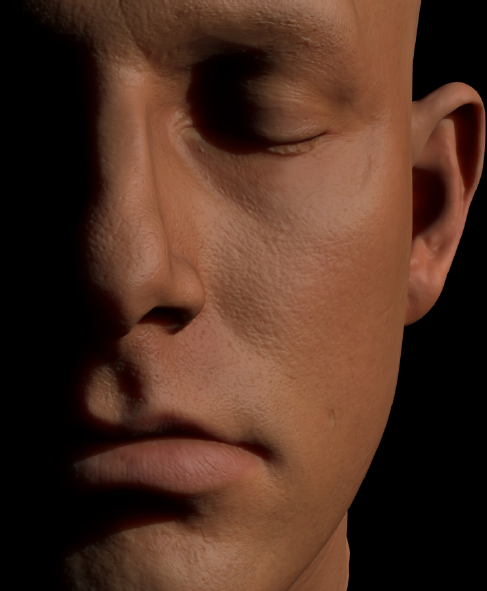
\includegraphics[scale=0.35,keepaspectratio]{./images/jensen-final-result.png}
    \caption{Ergebnis der BSSRDF von Donner und \\\hspace{\textwidth}Jensen\cite{spectral-bssrdf-human-skin}}
    \label{fig:outlook-bssrdf}
  \end{subfigure}%
  \begin{subfigure}{.5\textwidth}
    \centering
    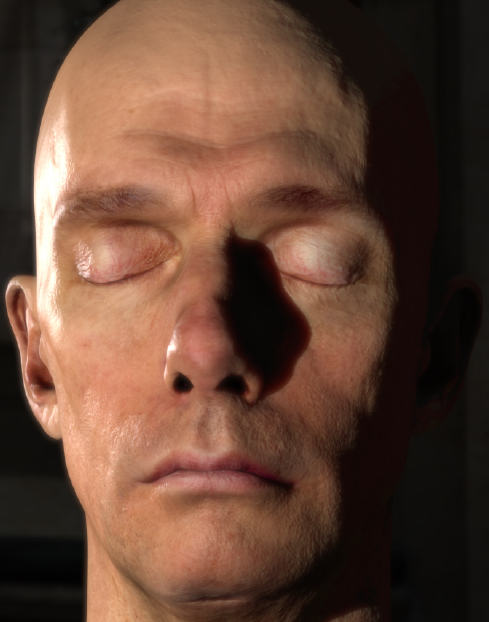
\includegraphics[scale=0.25,keepaspectratio]{./images/nvidia-result.jpg}
    \caption{Ergebnis der Texture-Space-Diffusion innerhalb eines Echtzeit-Renderers mit 2 Punkt-Lichtquellen, einer Umgebungslichtquelle und 2 teilbaren Bloomfiltern. Quelle: \cite{efficient-human-skin-rendering}}
    \label{fig:outlook-final-result}
  \end{subfigure}
\end{figure}

\begin{figure}
  \centering
  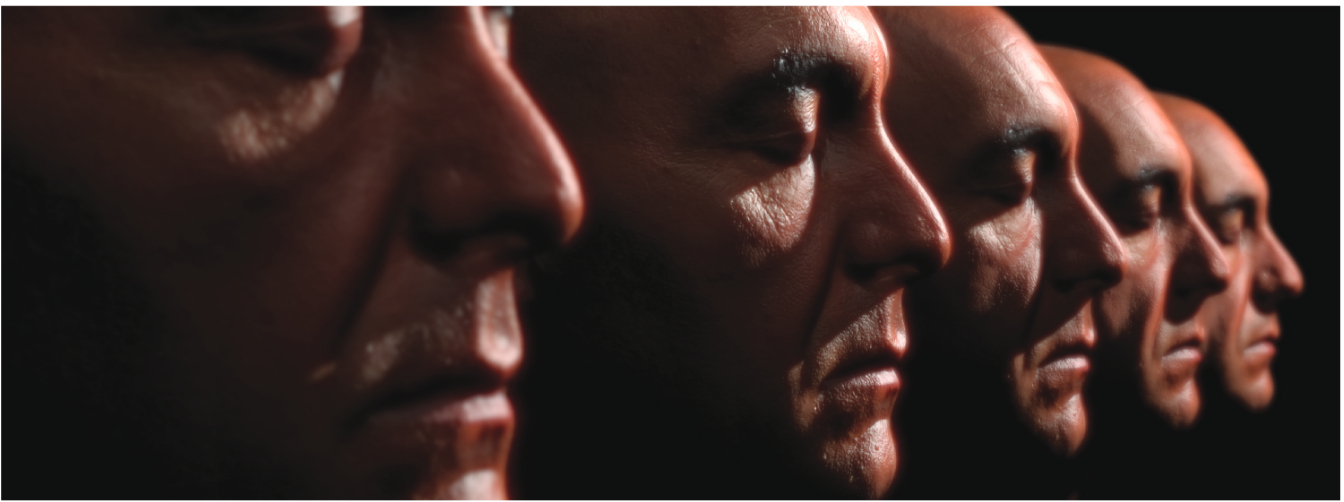
\includegraphics[scale=0.26,keepaspectratio]{./images/screen-space-sss.jpg}
  \caption{Ergebnis der Screen-Space-Variante des betrachteten Algorithmus.Quelle: \citet{screen-space-subsurface}}
  \label{fig:outlook-ssss}
\end{figure}

Zu hoffen bleibt jedoch, dass die Ergebnisse heutiger \enquote{Offline-Renderer} wie sie in den Grafiken \ref{fig:outlook-volumetric-path-tracer} und \ref{fig:outlook-monte-carlo-ray-tracer} zu sehen sind, in zukünftigen Echtzeitrenderer möglich werden.
Entweder durch Durchbrüche in der Forschung oder durch effizientere Consumer-Level-Hardware.
Die neue Grafikkarten-Reihe \enquote{Geforce RTX} von NVIDIA verwendet beispielsweise \enquote{Tensorprozessoren}, um eine Beschleunigung der \enquote{Ray Tracing}-Berechnungen zu erzielen \cite{forbes-tensor-rtx}.
möglicherweise wird dadurch Ray Tracing zukünftig eine gebräuchliche Technik für PCs.

\begin{figure}
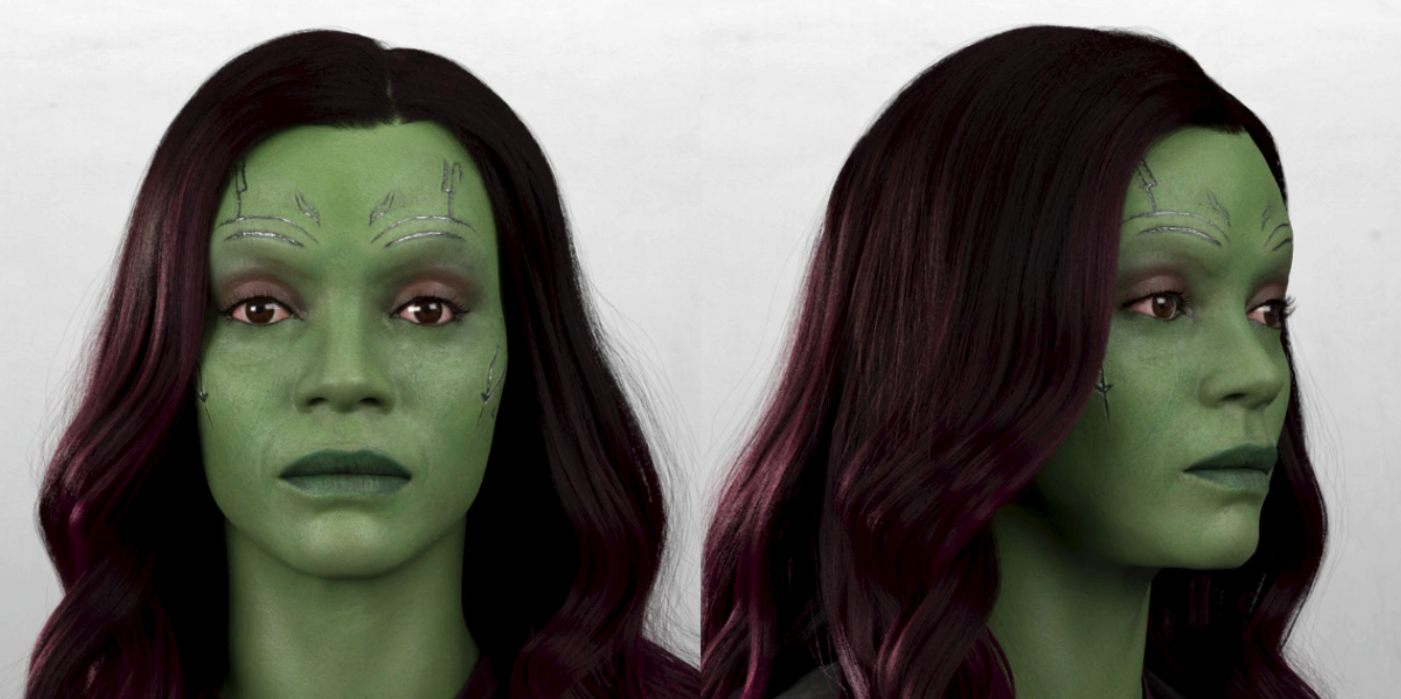
\includegraphics[scale=0.25,keepaspectratio]{./images/framestore-digital-gamora.jpg}
\caption{\enquote{Gamora} aus \enquote{Guardians of the Galaxy}, gerendert durch einen volumetrischen Path Tracer, der von Framestore, ein High-End VFX-Studio, entwickelt wurde. Sehr rechenintensiv, daher nicht für interaktives zurzeit verwendbar - Quelle: \cite{volumetric-path-tracer}}
\label{fig:outlook-volumetric-path-tracer}
\end{figure}

\begin{figure}
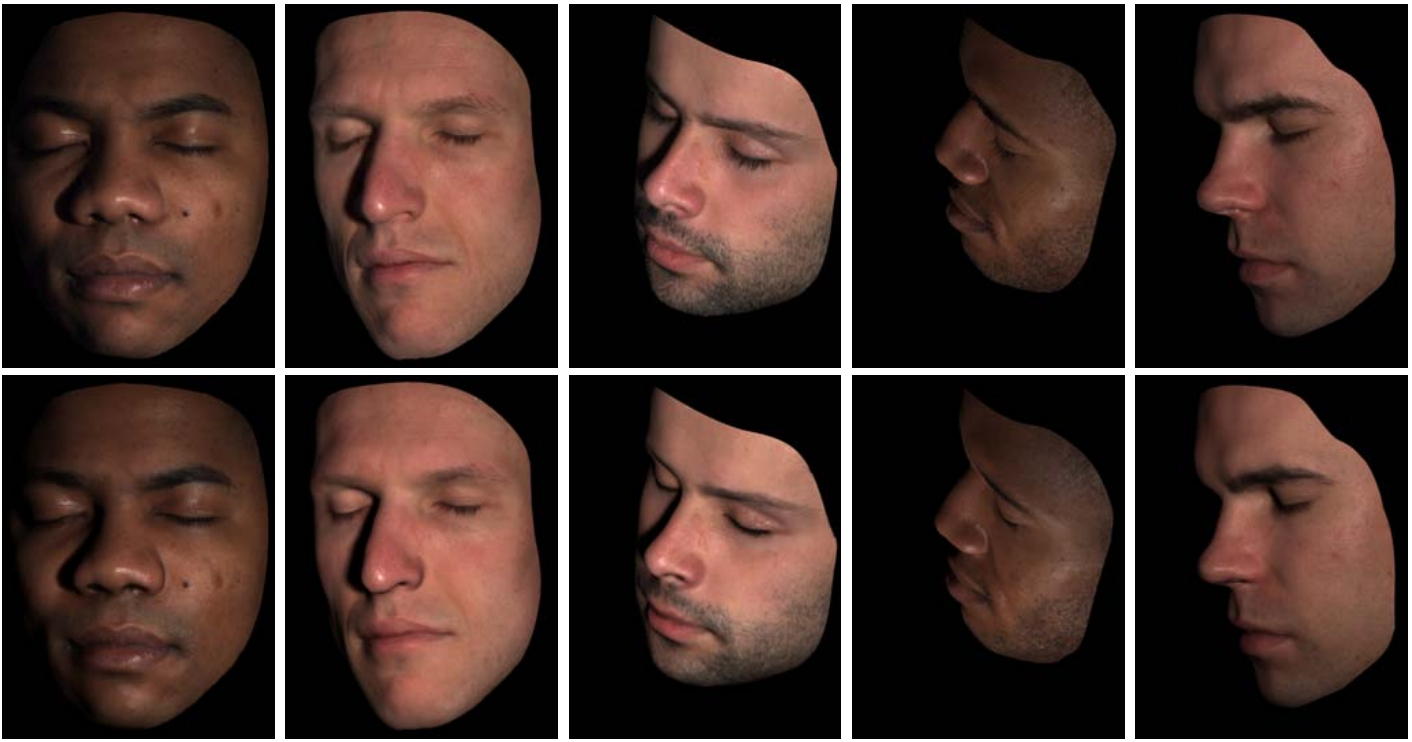
\includegraphics[scale=0.25,keepaspectratio]{./images/monte-carlo-ray-tracer.jpg}
\caption{Die Ergebnisse eines \enquote{Monte Carlo}-Raytracers implementiert in der Forschungsarbeit von \citet{weyrich2006analysis}.\\\hspace{\textwidth}In der oberen Reihe befinden sich die aufgenommenen Bilder, in der unteren Reihe die gerendereten Ergebnisse.}
\label{fig:outlook-monte-carlo-ray-tracer}
\end{figure}

\newpage

\renewcommand{\bibsection}{\section{Referenzen}} % requried for natbib to have "References" printed and as section, not chapter
% Use natbib compatbile splncsnat style.
% It does provide all features of splncs03, but is developed in a clean way.
% Source: http://phaseportrait.blogspot.de/2011/02/natbib-compatible-bibtex-style-bst-file.html
\bibliographystyle{splncsnat}
\begingroup
  \ifluatex
    %try to activate if bibliography looks ugly
    %\sloppy
  \else
    \microtypecontext{expansion=sloppy}
  \fi
  \small % ensure correct font size for the bibliography
  \bibliography{paper}
\endgroup

% Enforce empty line after bibliography
\ \\
%
Alle URLs wurden zuletzt am 21.05.2020 besucht.
\end{document}
